\documentclass{article} % For LaTeX2e
\usepackage{nips13submit_e,times}
\usepackage{hyperref}
\usepackage{url}
\usepackage{lipsum}
\usepackage{float}
\usepackage{listings}
\usepackage{booktabs}
\usepackage[pdftex]{graphicx} 
%\documentstyle[nips13submit_09,times,art10]{article} % For LaTeX 2.09


\title{Data Model}




\newcommand{\fix}{\marginpar{FIX}}
\newcommand{\new}{\marginpar{NEW}}

\nipsfinalcopy % Uncomment for camera-ready version

\begin{document}


\maketitle




\section{ER Diagram}

\begin{figure}[H]
	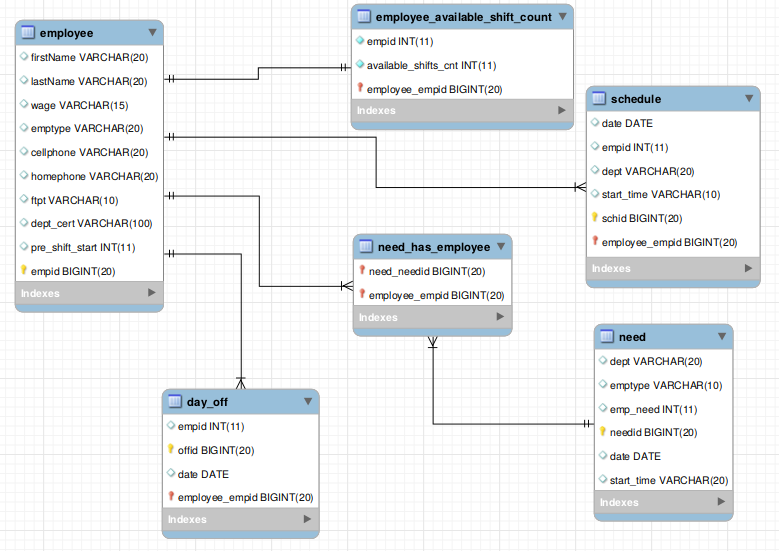
\includegraphics[height=12cm, width=16cm]{data_model.png}
	\caption{ER Diagram}
\end{figure}


\section{Tables Description}


\subsection*{DESCRIBE employee;}

\begin{table}[H]
	\centering
	\caption{\textbf{EMPLOYEE}}
\begin{tabular}{|p{2cm}|p{2cm}|p{2cm}|p{2cm}|p{2cm}|p{2cm}|p{2cm}|}
	\hline
	\toprule
	{} &            Field &                 Type & Null &  Key & Default &           Extra \\
	\hline
	\midrule
	0 &        firstName &          varchar(20) &  YES &      &    None &                 \\
	1 &         lastName &          varchar(20) &  YES &      &    None &                 \\
	2 &             wage &          varchar(15) &  YES &      &    None &                 \\
	3 &          emptype &          varchar(20) &  YES &      &    None &                 \\
	4 &        cellphone &          varchar(20) &  YES &      &    None &                 \\
	5 &        homephone &          varchar(20) &  YES &      &    None &                 \\
	6 &             ftpt &          varchar(10) &  YES &      &    None &                 \\
	7 &        dept\_cert &         varchar(100) &  YES &      &    None &                 \\
	8 &  pre\_shift\_start &              int(11) &  YES &      &    None &                 \\
	9 &            empid &  bigint(20) unsigned &   NO &  PRI &    None &  auto\_increment \\
	\bottomrule
	\hline
\end{tabular}
\end{table}


\subsection*{DESCRIBE need;}

\begin{table}[H]
	\centering
	\caption{\textbf{NEED}}
\begin{tabular}{|p{2cm}|p{2cm}|p{2cm}|p{2cm}|p{2cm}|p{2cm}|p{2cm}|}
	\hline
	\toprule
	{} &       Field &                 Type & Null &  Key & Default &           Extra \\
	\hline
	\midrule
	0 &        dept &          varchar(20) &  YES &      &    None &                 \\
	1 &     emptype &          varchar(10) &  YES &      &    None &                 \\
	2 &    emp\_need &              int(11) &  YES &      &    None &                 \\
	3 &      needid &  bigint(20) unsigned &   NO &  PRI &    None &  auto\_increment \\
	4 &        date &                 date &  YES &      &    None &                 \\
	5 &  start\_time &          varchar(20) &  YES &      &    None &                 \\
	\bottomrule
	\hline
\end{tabular}
\end{table}


\subsection*{DESCRIBE schedule;}


\begin{table}[H]
	\centering
	\caption{\textbf{SCHEDULE}}
\begin{tabular}{|p{2cm}|p{2cm}|p{2cm}|p{2cm}|p{2cm}|p{2cm}|p{2cm}|}
	\hline
	\toprule
	{} &       Field &                 Type & Null &  Key & Default &           Extra \\
	\hline
	\midrule
	0 &        date &                 date &  YES &      &    None &                 \\
	1 &       empid &              int(11) &  YES &      &    None &                 \\
	2 &        dept &          varchar(20) &  YES &      &    None &                 \\
	3 &  start\_time &          varchar(10) &  YES &      &    None &                 \\
	4 &       schid &  bigint(20) unsigned &   NO &  PRI &    None &  auto\_increment \\
	\bottomrule
	\hline
\end{tabular}
\end{table}


\subsection*{DESCRIBE day\_off;}
\begin{table}[H]
	\centering
	\caption{\textbf{DAY OFF}}
\begin{tabular}{|p{2cm}|p{2cm}|p{2cm}|p{2cm}|p{2cm}|p{2cm}|p{2cm}|}
	\hline
	\toprule
	{} &  Field &                 Type & Null &  Key & Default &           Extra \\
	\hline
	\midrule
	0 &  empid &              int(11) &  YES &      &    None &                 \\
	1 &  offid &  bigint(20) unsigned &   NO &  PRI &    None &  auto\_increment \\
	2 &   date &                 date &  YES &      &    None &                 \\
	\hline
	\bottomrule
\end{tabular}
\end{table}


\subsection*{DESCRIBE employee\_available\_shift\_count;}

\begin{table}[H]
	\centering
	\caption{\textbf{EMPLOYEE AVAILABLE SHIFT}}
\begin{tabular}{|p{2cm}|p{2cm}|p{2cm}|p{2cm}|p{2cm}|p{2cm}|p{2cm}|}
	\hline
	\toprule
	{} &                 Field &     Type & Null & Key & Default & Extra \\
	\hline
	\midrule
	0 &                 empid &  int(11) &   NO &     &    None &       \\
	1 &  available\_shifts\_cnt &  int(11) &   NO &     &    None &       \\
	\hline
	\bottomrule
\end{tabular}
\end{table}


\end{document}
